\documentclass[10pt, conference, a4paper, final]{IEEEtran}
\IEEEoverridecommandlockouts
% For better handling of math expressions
\usepackage{amsmath}

% For better formatting of lists
\usepackage{enumitem}

% Optional for improved typography
\usepackage{microtype}
\usepackage[margin=1in]{geometry} % Adjust margins as needed
\usepackage{lipsum} % Provides sample text. Remove this for your actual document.
\usepackage[table,xcdraw]{xcolor}
\usepackage{colortbl}
\usepackage{graphicx} % Required for including images
\usepackage{graphicx}
\usepackage{textcomp}
\usepackage{xcolor}
\usepackage{float}
\usepackage{amsmath}
\usepackage{longtable}
\usepackage{booktabs}
\usepackage{multicol}
\usepackage{multirow}
\usepackage[margin=0.7in]{geometry}
\usepackage{array}
\usepackage{hyperref}
\usepackage{relsize, fullpage, url, array}
\usepackage{lscape, afterpage}
\usepackage{float,lscape}
\usepackage{algorithm}
\usepackage{algorithmic}  
\usepackage[algo2e]{algorithm2e} 
\usepackage{amsmath}
\usepackage{mathtools}
\usepackage{tabularx}
\usepackage{algorithmic}
\usepackage{graphicx}
\usepackage{textcomp}
\usepackage{xcolor}
\title{Adversarial Attack}
\author{Arooj Arif}
\date{\today} % You can also specify a date manually

\begin{document}

\maketitle % This command creates the title

\section{Problem Statement}

Deep learning technologies have become integral in critical domains like healthcare and autonomous driving, offering significant advancements in tasks such as image recognition and decision-making. However, this increasing reliance also introduces substantial security challenges, particularly the vulnerability of these systems to adversarial attacks. Such vulnerabilities are a major concern in sectors where accuracy and reliability are paramount.

The core problem lies in the potential of deep learning systems to be compromised, leading to erroneous decisions or actions with severe consequences. For instance, a healthcare diagnostic system misidentifying a disease due to an adversarial attack could result in incorrect treatment, while an autonomous vehicle misinterpreting road signs could lead to accidents. These risks underline the necessity of comprehensively understanding and mitigating the threats posed by different types of adversarial attacks.

Particularly, the study focuses on evaluating the practicality and effectiveness of white-box adversarial attacks, where attackers have complete knowledge of the neural network model, in comparison to other adversarial paradigms. This comparison is critical in determining the real-world applicability of these attacks and in developing robust defense mechanisms. Ensuring the security and integrity of deep learning systems in these high-stakes applications is crucial for maintaining public trust in this rapidly evolving technology.

\section{Motivation}

The motivation for addressing the security challenges in deep learning models is twofold:

\begin{enumerate}
    \item \textbf{Protecting Critical Applications}: The increasing deployment of deep learning in critical areas such as healthcare and transportation demands rigorous security measures. This research emphasizes the need to understand and mitigate specific threats posed by different types of adversarial attacks, including the theoretically rigorous but practically challenging white-box attacks. Ensuring the robustness of these systems against a diverse range of attacks is vital for preventing errors that could have severe consequences on patient care, road safety, and public trust in advanced technologies.
    
    \item \textbf{Advancing Deep Learning Technology Through Security Insights}: By examining and contrasting the effectiveness of various adversarial attack paradigms, this study seeks to advance the field of deep learning. It aims to provide insights into the relative strengths and weaknesses of different attack strategies, particularly focusing on the gap between theoretical attack models like white-box attacks and their real-world applicability. Such understanding is crucial for developing more resilient and reliable AI technologies that can withstand sophisticated cyber threats in a range of environments.
\end{enumerate}


\section{Threat Model}

We discuss in this section how to model threats against the mentioned attacks. We define the attacker’s goal, knowledge, and capability of manipulating the input data, to subsequently define an optimization problem corresponding to the optimal attack strategy, which we mainly base on the discussion by Biggio and Roli (2018) \cite{BR18}. The solution to this problem provides a way to manipulate input data to achieve the attacker’s goal.

\subsection{Attacker’s Goal}

The attacker’s goal is defined in the following terms:

\begin{itemize}
    \item \textbf{Security violation.} The attacker may aim to cause: an integrity violation, i.e., to evade detection without compromising normal system operation; an availability violation, i.e., to compromise the normal system functionalities available to legitimate users; or a privacy violation, to obtain private information about the system, its users, or data by reverse-engineering the learning algorithm. Integrity, availability, and confidentiality are also known as the CIA triad and represent the fundamental principles of information security \cite{Perrin}.
    
    \item \textbf{Attack specificity.} The attack can be either targeted or untargeted. Targeted attacks aim to cause the model to misclassify a specific set of samples (to target a given system user or protected service), while with the untargeted attacks the attacker aims to cause misclassification of any sample (to target any system user or protected service).
    
    \item \textbf{Error specificity.} It can be either specific if the attacker aims to have a sample misclassified as a specific class; or generic, if the attacker aims to have a sample misclassified as any of the classes different from the true class.
\end{itemize}

\subsection{Attacker’s Knowledge}

Additionally, different attack scenarios can be described based on the attacker’s knowledge of the targeted system. This includes different levels of knowledge such as the training data, the feature set, the learning algorithm along with the objective function and possibly even its trained hyper-parameters.

\begin{itemize}
    \item \textbf{White-box setting} - attacker is assumed to know everything about the targeted system.
    \item \textbf{Gray-box setting} - attacker is assumed to know something about the targeted system.
    \item \textbf{Black-box setting} - attacker is assumed to know nothing about the targeted system.
\end{itemize}


\begin{figure*}[!ht]
\centering
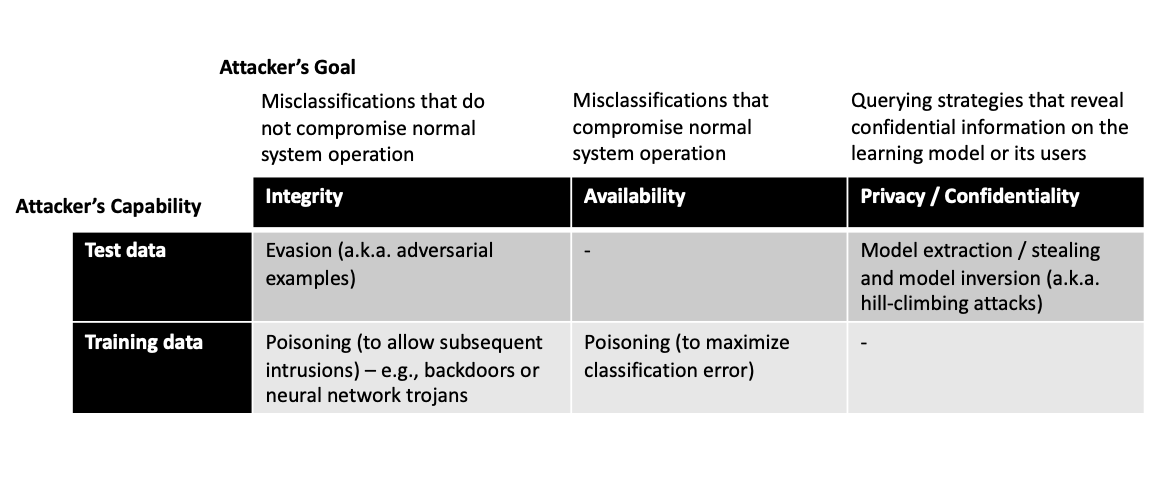
\includegraphics[width=1\textwidth]{proposal_images/attackergoal_capability.png}
\caption{Summary of Attacker Capability and Attacker Goal}
\label{threat model}
\end{figure*}
\subsection{Attacker’s Capability}

This characteristic depends on the influence that the attacker has on the input data and application-specific data manipulation constraints.

\begin{itemize}
    \item \textbf{Attack influence.} It can be causative if the attacker can manipulate both training and test data, or exploratory if the attacker can only manipulate test data. These scenarios are more commonly known as poisoning and evasion attacks.
    
    \item \textbf{Data manipulation constraints.} Another aspect related to the attacker’s capability depends on the presence of application-specific constraints on data manipulation. For example, to evade malware detection, malicious code has to be modified, but without compromising its intrusive functionality.
\end{itemize}

\begin{figure*}[!ht]
\centering
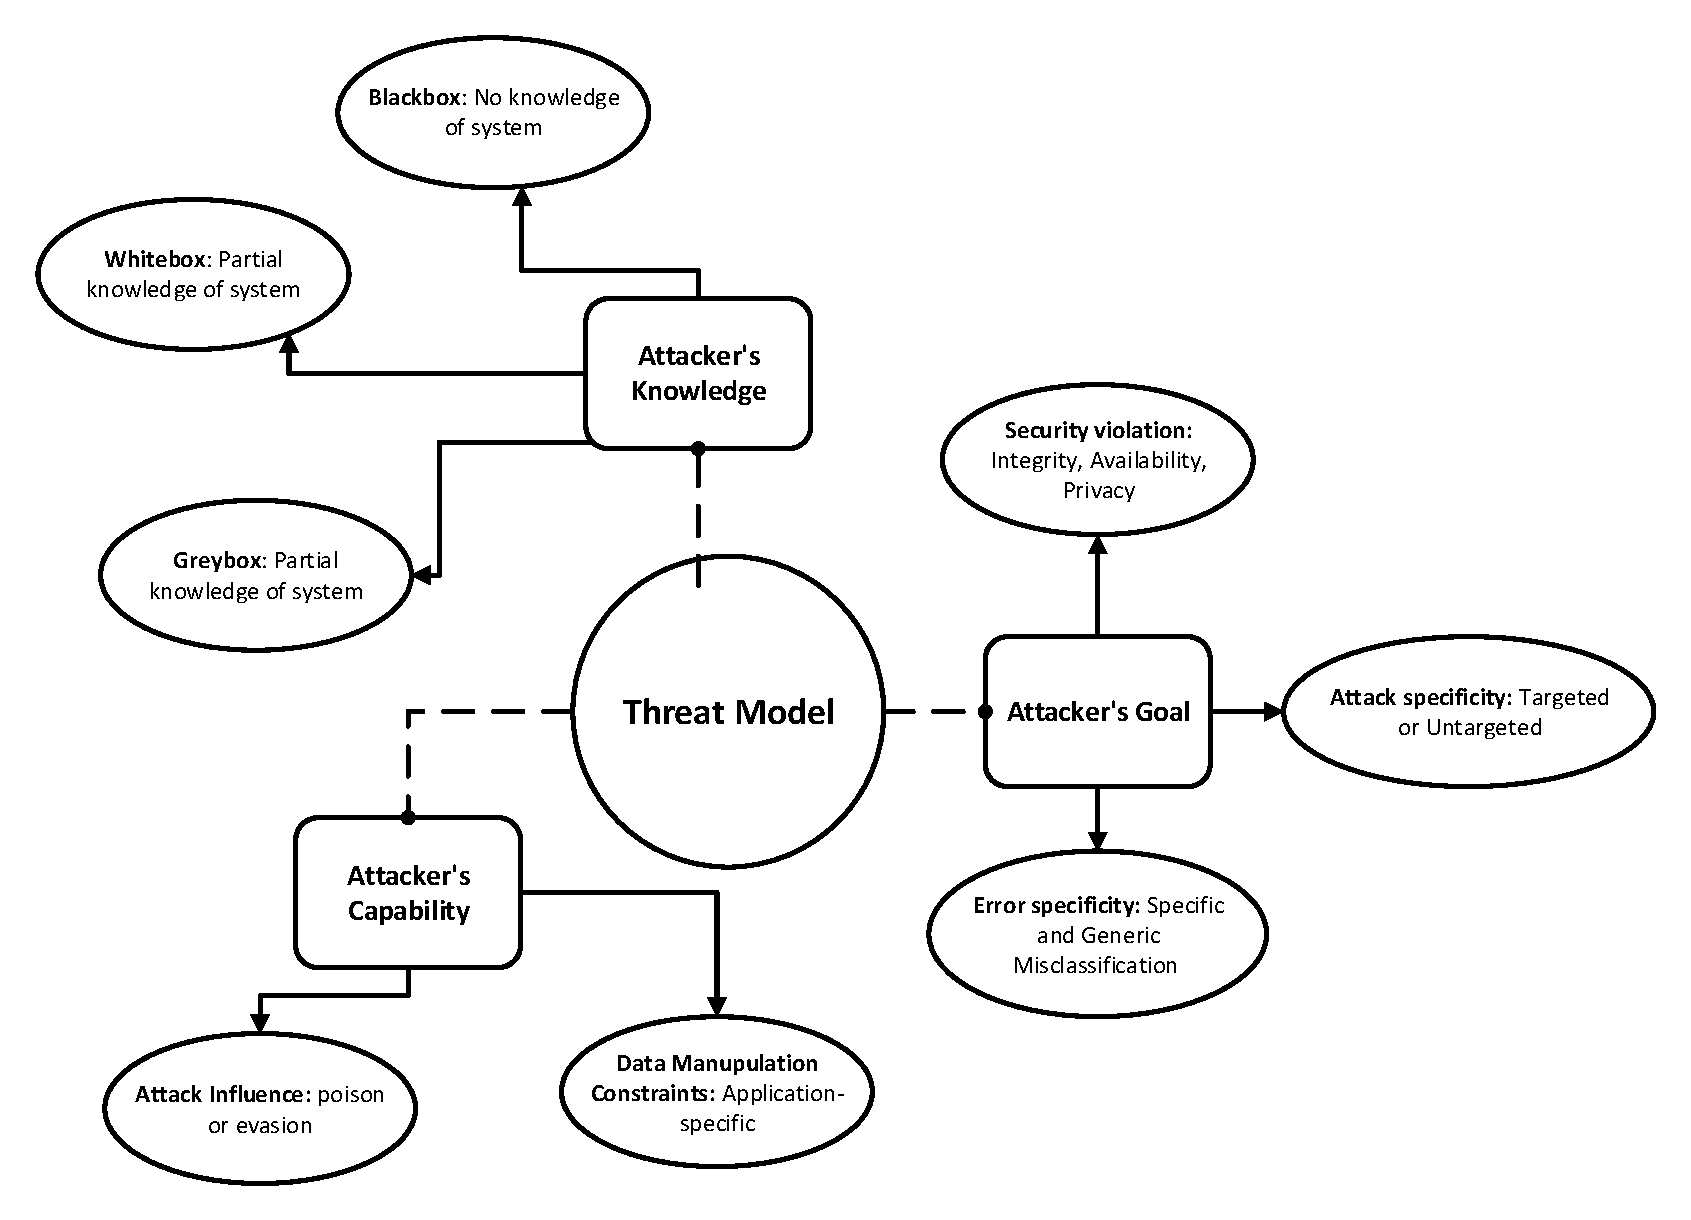
\includegraphics[width=1\textwidth]{proposal_images/Threatmodel.pdf}
\caption{Threat Model}
\label{threat model}
\end{figure*}


\subsection{Common Terms}

The adversarial attack is to attack the deep neural network through the adversarial example. According to the characteristics and attack effect of the adversarial attack, the adversarial attack can be divided into black-box attack and white-box attack, one-shot attack and iterative attack, targeted attack and non-targeted attack, specific perturbation and universal perturbation, etc., the terms are introduced as follows:

\begin{description}
    \item[Black-box attack:] The attacker cannot access the deep neural network model, and thus cannot obtain the model structure and parameters, and can only obtain the output result of the target model by inputting the original data to the target model.
    \item[White-box attack:] The attacker can obtain the complete structure and parameters of the target model, including training data, gradient information, and activation functions, etc.
    \item[One-step attack:] The adversarial attack algorithm only needs to perform one calculation to obtain an adversarial example with a high attack success rate.
    \item[Iterative attack:] The adversarial attack algorithm needs to be run multiple times to generate adversarial examples. Compared with the one-shot attack, the iterative attack takes a longer running time but has a better attack effect.
    \item[Targeted attack:] After the adversarial examples designed by the attacker are input into the target model, the target classifier can misjudge the specified classification result.
    \item[Un-targeted attack:] The adversarial example only needs to be misjudged by the target classifier, and does not limit the classification result.
    \item[Specific perturbation:] Add different perturbations to each input original data to form different perturbation patterns.
    \item[Universal perturbation:] The same perturbation is added to each input original data, and its perturbation mode is the same.
  \item [$L_0$ Norm:] Measures the number of elements of a vector that are different from zero. In adversarial attacks, it represents the number of altered pixels in an image, aiming to change as few pixels as possible.
    \item[$L_2$ Norm:] Also known as the Euclidean norm, it measures the Euclidean distance between the original and the perturbed input. It represents the root mean square difference between the pixel values of the original and adversarial image.
    \item [$L_{\infty}$ Norm:] Measures the maximum change to any element of the input vector. For images, this is the largest change to any pixel value. It limits the maximum perturbation allowed for each pixel.
\end{description}



Each norm provides a different perspective on the perturbation:
\begin{itemize}
    \item $L_0$ focuses on the number of changes.
    \item $L_2$ considers the overall magnitude of the change.
    \item $L_{\infty}$ limits the maximum allowed change per element.
\end{itemize}


\begin{table*}[!ht]
    \centering
    \caption{Summary of Whitebox Adversarial Attacks}
    \label{tab:attacks_properties}
    \normalsize
    \setlength\extrarowheight{1pt}
    \resizebox{\linewidth}{!}{
        \begin{tabular}{|l|l|l|l|}
            \hline
            \rowcolor[HTML]{FFCE93}
            \textbf{Methods} & \textbf{Attack goal} & \textbf{Attack frequency} & \textbf{Perturbation norm} \\ \hline
            L-BFGS\cite{Christian}           & Targeted             & Iterative                 & $L_{\infty}$                \\ \hline
            FGSM \cite{Ian}            & Targeted/untargeted  & One-step                  & $L_{\infty}$                \\ \hline
            BIM \cite{Alexey}              & Targeted/untargeted  & Iterative                 & $L_{\infty}$                \\ \hline
            PGD\cite{Aleksander}               & Targeted/untargeted  & Iterative                 & $L_{\infty}$                \\ \hline
            MI-FGSM/MIM\cite{Yinpeng}       & Targeted/untargeted  & Iterative                 & $L_{\infty}$                \\ \hline
            NI-FGSM \cite{Jiadong}          & Untargeted           & Iterative                 & $L_{\infty}$                \\ \hline
            JSMA \cite{Nicolas}             & Targeted/untargeted  & Iterative                 & $L_0$                       \\ \hline
            Deepfool\cite{Seyed}          & Untargeted           & Iterative                 & $L_2$, $L_{\infty}$         \\ \hline
            UAP \cite{Seyed}              & Untargeted           & Iterative                 & $L_2$, $L_{\infty}$         \\ \hline
            C\&W \cite{Carlini}             & Targeted/untargeted  & Iterative                 & $L_0$, $L_2$, $L_{\infty}$  \\ \hline
            LogBarrier \cite{Chris}       & Untargeted           & Iterative                 & $L_{\infty}$                \\ \hline
        \end{tabular}
    }
\end{table*}

\begin{figure*}[!ht]
\centering
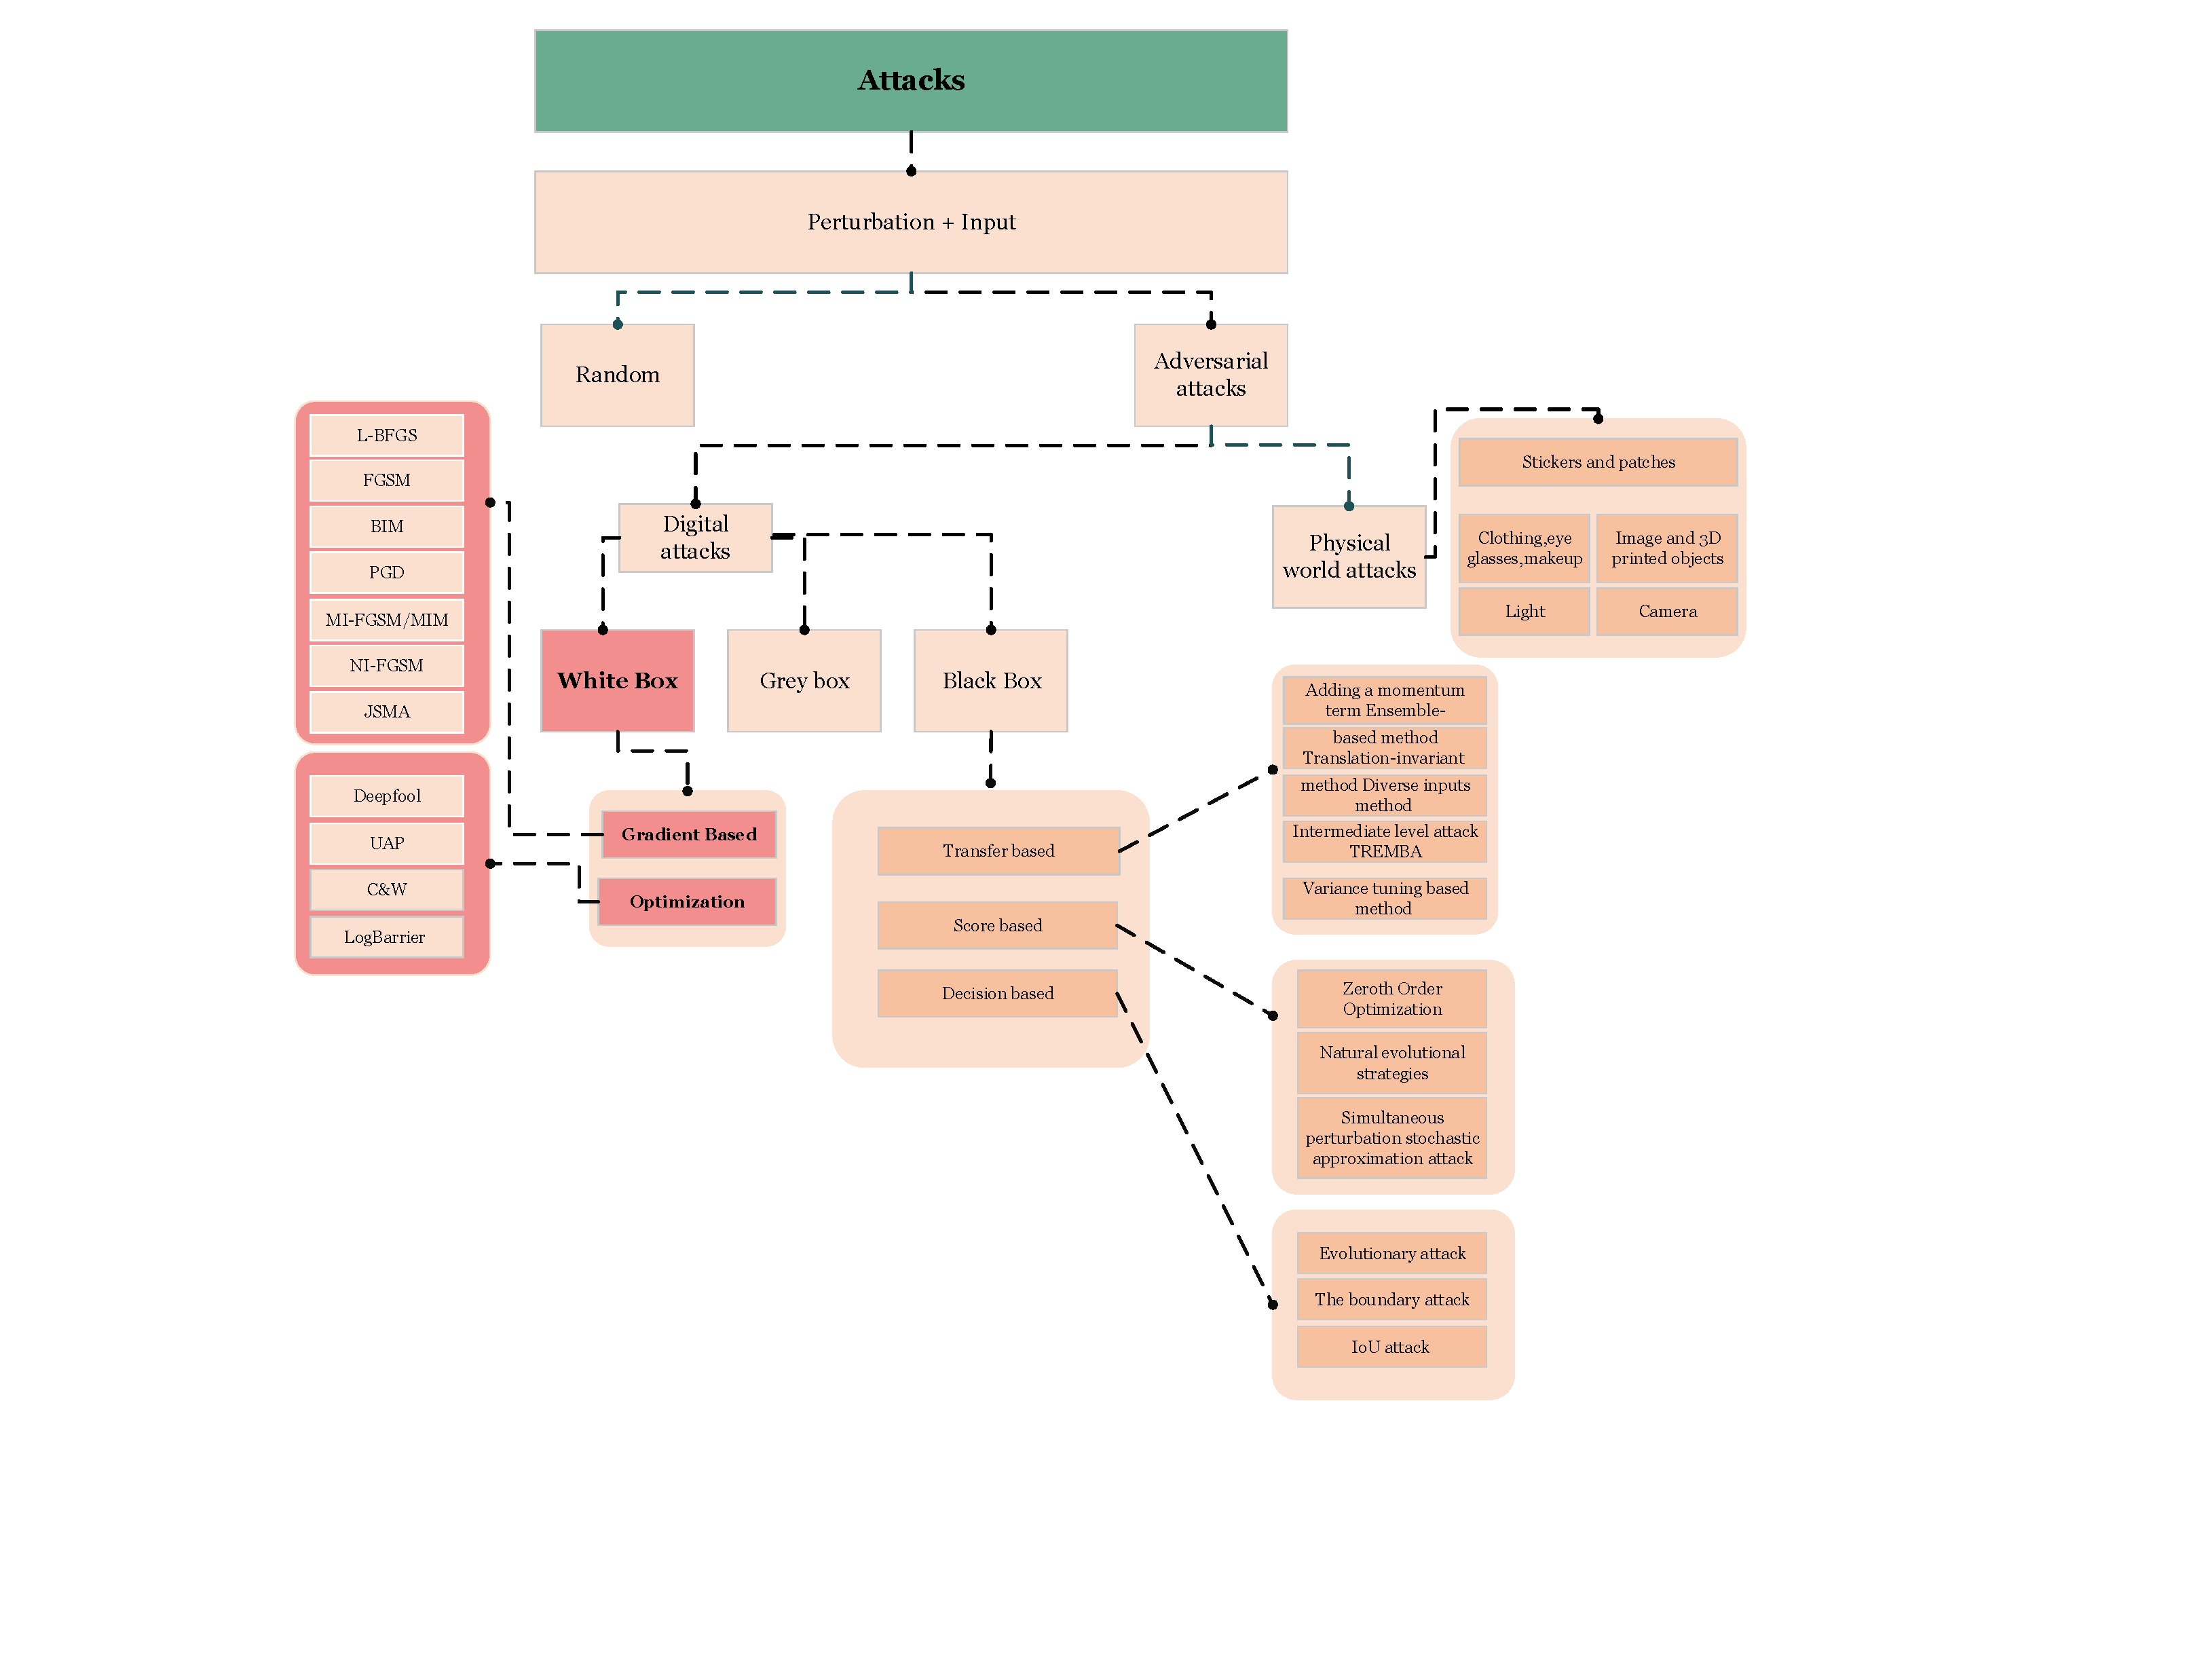
\includegraphics[width=1.3\textwidth]{proposal_images/AttacksFlowchart.pdf}
\caption{Comprehensive Diagram of Attacks}
\label{threat model}
\end{figure*}

\section{Examination of White Box Testing Paradigms in Deep Learning Security Frameworks}

The primary focus of this research is to thoroughly examine white box testing within deep learning security frameworks. This involves a comprehensive exploration of adversarial attacks, especially those conducted in a white-box setting where the attacker has full knowledge of the neural network, including its structure and parameters. Such testing is pivotal in cybersecurity for uncovering latent vulnerabilities that are not apparent in less-informed testing scenarios.

\subsection{Introduction to Adversarial Attacks in Deep Learning}

We begin by contextualizing adversarial attacks within the realm of deep learning, underscoring their impact on the reliability and safety of critical AI applications. This overview sets the stage for a deeper investigation into specific attack methodologies.

\subsection{Overview and Contextualization of Evasion and White-Box Attacks}

Evasion attacks, which subtly alter input data during the inference phase to mislead the model, are introduced as a key focus of this study. We then transition to discussing white-box attacks as a specialized category within evasion attacks, characterized by the attacker's comprehensive understanding of the model.

\subsection{Exploring Types of White-Box Attacks}

Gradient-Based Attacks: Our investigation delves into gradient-based attacks, where the attacker exploits the model's gradient information to craft perturbations, a technique we have actively implemented and analyzed.

Optimization-Based Attacks: We also explore optimization-based attacks, utilizing complex optimization algorithms to identify effective perturbations, providing a contrasting approach to gradient-based methods.

\subsection{Evasion Attacks and Electricity Theft in Smart Grids: A Case Study}
Evasion attacks in smart grids, particularly in the context of electricity theft, represent a critical challenge to grid security and stability. Smart grids, integrating advanced metering infrastructures (AMI) with machine learning algorithms for monitoring and control, are vulnerable to such attacks where malicious entities manipulate data or meter readings. These evasion attacks, often undetected, lead to incorrect grid decisions, causing financial losses and jeopardizing grid integrity. A notable instance is when attackers alter consumption data, mimicking legitimate user patterns, to steal electricity. This not only results in direct revenue losses but also destabilizes the load distribution across the grid, potentially leading to larger-scale disruptions. The sophistication of these attacks necessitates advanced detection methods, such as deep learning models, which can discern between genuine consumption patterns and those altered by evasion techniques. Implementing robust, intelligent systems for early detection and prevention of such fraudulent activities is imperative for ensuring the resilience and reliability of smart grids against evasion attacks and electricity theft 

 % Please add the following required packages to your document preamble:
% \usepackage[table,xcdraw]{xcolor}
% Beamer presentation requires \usepackage{colortbl} instead of \usepackage[table,xcdraw]{xcolor}



\begin{thebibliography}{01}
	% \bibitem{JiangR.}
	% Jiang, R., Lu, R., Wang, Y., Luo, J., Shen, C. and Shen, X., 2014. Energy-theft detection issues for advanced metering infrastructure in smart grid. Tsinghua Science and Technology, 19(2), pp.105-120.
\bibitem{BR18}	
Battista Biggio and Fabio Roli. Wild patterns: Ten years after the rise of adversarial machine learning. Pattern Recognition, 84:317–331, 2018.
\bibitem{Perrin}
Chad Perrin. The cia triad. Dostopno na: http://www. techrepublic. com/blog/security/the-cia-triad/488, 2008.

    \bibitem{Christian} 
   Christian Szegedy, Wojciech Zaremba, Ilya Sutskever, Joan Bruna, Dumitru Er- han, Ian J. Goodfellow, Rob Fergus, Intriguing properties of neural networks, in: Yoshua Bengio, Yann LeCun (Eds.), 2nd International Conference on Learning Representations, ICLR 2014, Banff, AB, Canada, April 14-16, 2014, Conference Track Proceedings, 2014.
    
    \bibitem{Ian}
   Ian J. Goodfellow, Jonathon Shlens, Christian Szegedy, Explaining and harnessing adversarial examples, in: International Conference on Learning Representations, 2015.
   \bibitem{Alexey} 
   Alexey Kurakin, Ian Goodfellow, Samy Bengio, Adversarial examples in the physical world, 2016, arXiv preprint arXiv:1607.02533.
\bibitem{Aleksander}
Aleksander Madry, Aleksandar Makelov, Ludwig Schmidt, Dimitris Tsipras, Adrian Vladu, Towards deep learning models resistant to adversarial attacks, in: International Conference on Learning Representations, 2018.
\bibitem{Yinpeng}
Yinpeng Dong, Fangzhou Liao, Tianyu Pang, Hang Su, Jun Zhu, Xiaolin Hu, Jianguo Li, Boosting adversarial attacks with momentum, in: Proceedings of the IEEE Conference on Computer Vision and Pattern Recognition, 2018, pp. 9185–9193.
\bibitem{Jiadong}
Jiadong Lin, Chuanbiao Song, Kun He, Liwei Wang, John E Hopcroft, Nesterov accelerated gradient and scale invariance for adversarial attacks, 2019, arXiv preprint arXiv:1908.06281.
\bibitem{Nicolas}
Nicolas Papernot, Patrick McDaniel, Somesh Jha, Matt Fredrikson, Z Berkay Ce- lik, Ananthram Swami, The limitations of deep learning in adversarial settings, in: 2016 IEEE European Symposium on Security and Privacy, (EuroS\&P), IEEE, 2016, pp. 372–387.
\bibitem{Seyed}
Seyed-Mohsen Moosavi-Dezfooli, Alhussein Fawzi, Pascal Frossard, Deepfool: A simple and accurate method to fool deep neural networks, in: Proceedings of the IEEE Conference on Computer Vision and Pattern Recognition, 2016, pp. 2574–2582.
\bibitem{Carlini}
Nicholas Carlini, David Wagner, Towards evaluating the robustness of neural networks, in: 2017 IEEE Symposium on Security and Privacy, (SP), IEEE, 2017, pp. 39–57.
\bibitem{Chris}
Chris Finlay, Aram-Alexandre Pooladian, Adam Oberman, The logbarrier ad- versarial attack: making effective use of decision boundary information, in: Proceedings of the IEEE/CVF International Conference on Computer Vision, 2019, pp. 4862–4870.

\end{thebibliography}
\end{document}
